%%%%%%%%%%%%%%%%%%%%%%%%%%%%%%%%%%%%%%%%%

\documentclass[]{cv} % Add 'print' as an option into the square bracket to remove colors from this template for printing

\geometry{left=4.5cm,top=3cm,right=4.5cm,bottom=3cm,nohead,nofoot}

\def\firstname{Benjamin}
\def\familyname{Vial}
\def\FileSubject{cover letter}
\def\FileAuthor{\firstname~\familyname}
\def\FileTitle{\firstname~\familyname's~\FileSubject}
\def\FileKeyWords{\firstname~\familyname, \FileSubject}



  \RequirePackage[unicode]{hyperref}% unicode is required for unicode pdf metadata
  \hypersetup{
    breaklinks,
    baseurl       = http://,
    pdfborder     = 0 0 0,
    pdfpagemode   = UseNone,% do not show thumbnails or bookmarks on opening
    pdfstartpage  = 1,
%    pdfproducer   = {\LaTeX{}},% will/should be set automatically to the correct TeX engine used
    bookmarksopen = true,
    bookmarksdepth= 2,% to show sections and subsections
    pdfauthor   = {\FileAuthor},%
    pdftitle    = {\FileTitle},%
    pdfsubject  = {\FileSubject},%
    pdfkeywords = {\FileKeyWords},%
    pdfcreator  = {\LaTeX},%
    pdfproducer = {\LaTeX}
    }

    

\begin{document}
\hfill%
\begin{minipage}[t]{.6\textwidth}
\raggedleft{\bfseries Benjamin Vial}\\
146 Glyn Road\\
London E5 0JE, UK\\
\faPhone~~+44~7840~029~744\\
\faEnvelope~~\href{mailto:b.vial@qmul.ac.uk}{b.vial@qmul.ac.uk}\\
\faUser~~\href{www.bvial.info}{bvial.info}
\\[2em]
\today
\end{minipage}\\[1em]
\begin{minipage}[t]{.4\textwidth}
    \begin{flushleft}
        \textbf{Queen Mary, University of London}\\
Personnel dept.\\
Mile End Road\\
London E1 4NS
    \end{flushleft}
\end{minipage}
\hfill % US style
\\[2em]
%\raggedright
\textbf{Object:} Application to the post of Lecturer in Quantum and Terahertz Experimental Electronic
Systems (Teaching and Research)\\[1.5em]

Dear Professor Uhlig,\\[1em]


I am pleased to attach my CV and application form for the post of Senior
Lecturer in French History as advertised on the jobs.ac.uk website.

For the past five years I have held the post of Lecturer in the department
of French Studies at the University of Northtown, where my research
has focused primarily on Eighteenth and Nineteenth Century French
Atlantic history. I have a particular interest in the history of the Haitian
revolution and have recently developed a new undergraduate module
in Post Colonial Caribbean History in collaboration with the department
of History and the department of Hispanic Studies.

I have published widely in the field of French Atlantic history and society.
My monograph, “Piracy and Revolution in the Lesser Antilles” won the
Leverhulme award and I was invited to become a Fellow of the Royal
Historical Society. My research received outstanding peer reviews
and helped the department attain a 4* rating in the 2008 Research
Assessment Exercise.

Currently I am researching the history of the great planter families
in Tortuga in the early nineteenth century and their links with the
Haitian Revolution, for which I have been awarded a two year grant
from the Arts and Humanities Research Council. My enquiry focuses
on the transition from autocratic and feudal structures to democratic
institutions in the French Atlantic and the cultural barriers to democracy
in post-colonial societies. It examines transatlantic family structures
and their influence on French and Colonial political life. I have been
fortunate to spend a six month sabbatical at the Universite d’Etat d’Haiti
where I was able to conduct primary research with officials in the Haitian
government and the United Nations. This has resulted in a six month
consultancy project from the Haitian Ministry of Social Justice to advise
on electoral reform.

I believe my research has clear links with your Post Colonial French
History research group and would contribute well to your joint degrees
with the Sociology and History departments, for example your modules
in Nineteenth Century French Caribbean History and Slave Societies
in Eighteenth Century French Colonies.

Having discussed my research interests with Dr Benoit and Dr Ward,
I was impressed by the close integration of research and teaching in
the department. I am passionate about the value of integrating doctoral
research into undergraduate teaching and recently introduced a
programme for PhD students to supervise and mentor undergraduates
during their final year dissertations.

I am also impressed by the strength of your e-learning platforms and
believe I can help develop these further. As placement officer for the
year abroad I extended our e-learning resources to provide support
from Language Assistants to students during their second year
overseas. This received excellent feedback in our departmental
Student Experience Survey.

I currently teach undergraduate modules on French Atlantic History
1790 – 1840 and The Haitian Revolution and its Links to French
Political Life and can also offer both undergraduate and postgraduate
modules on Twentieth Century French Caribbean Politics, Francophone
Slave Literature and French Caribbean Language and Dialects. I currently
supervise three PhD students and have seen two of my PhD students
receive their awards this year.

In addition to my teaching and supervision duties, I serve on the Staff
Student Liaison Group. From 2009 - 2011 I acted as Undergraduate
Admissions Tutor for the department; a period which saw an 8% rise
in applications at a time when applications nationally dipped by 5%.
This was achieved by implementing a new schools outreach programme
and improving communications with prospective students at the
post-offer stage.

As associate editor of the ‘French Atlantic Political Review’ I have
organised a number of conferences. This included a conference on
‘Electoral Reform in the French Caribbean’ in Haiti in April which was
attended by 350 delegates and where I was one of the keynote speakers.
In summary, I believe my relevant expertise in French Atlantic history,
politics and society, my strong research and publications record, my
ability to support the department’s joint degree programmes and my
achievements in integrating research and teaching whilst improving the
student experience make me ideally placed to contribute in this Senior
Lecturer position.

I look forward to the opportunity to discuss my application further at
interview. Please contact me if you would like any further information
in the meantime.




% I am writing to apply for the postdoctoral position ``The Quest for Ultimate Electromagnetics using Spatial Transformations (QUEST)''
% as an answer to the call 
% found on \emph{Queen Mary University} website. I am currently a postdoctoral fellow at \emph{Institut Fresnel} (Marseille,
% France) under the direction of Dr. Nicolas Bonod, and fully completed my PhD in last April. I am
% extremely interested in obtaining a position in your \emph{Antennas and Electromagnetics research group}, as its
% electromagnetics research programs have a stellar reputation that is
% known worldwide.
% 
% I believe that my engineering/master degree at \emph{\'Ecole Centrale Marseille}
% followed by three years of PhD, in academia at 
% \emph{Institut Fresnel} under the direction of Prof. Mireille Commandr\'e
% and in industry at \emph{Silios Technologies} under the direction of Dr. St\'ephane Tisserand, 
% prepare me to be an effective researcher in 
% your group and more specifically on this project. During my PhD, I have developed in collaboration with the CLARTE team
% (Pr. Fr\'ed\'eric Zolla and Pr. Andr\'e Nicolet)
% a systematic approach based on the Finite Element Method 
% to study resonances in bi-periodic open electromagnetic structures,
% \textit{i.e.} finding complex eigenfrequencies and leaky eigenmodes 
% of Maxwell's operator. Through a geometrical 
% transformation of space, our method allows to treat a bounded problem where the free space is truncated by 
% Perfectly Matched Layers (PML).
% The main advantage of this method is its complete generality with
% respect to the studied geometries and the material properties. 
% In addition, I have developed adaptive PMLs (APMLs) with an \textit{ad hoc} transformation of coordinate
%  to treat the case of Wood's anomalies 
% for which the classical PMLs become ineffective when dealing with the diffraction of a plane wave by a grating. 
% I also developed a technique to study the conditions of excitation of the modes of the periodic and non periodic structures. 
% By expanding an electromagnetic field solution of Maxwell's equations with sources on the eigenmode basis, 
% the method reveals the relative importance of the different photonic states in the scattering process. 
% I successfully applied these methods to find a set of opto-geometrical parameters
% for crossed-gratings that realize different filtering functions in the thermal infrared.
%  Finally, I supervised the fabrication of these nano-structures 
% including vacuum evaporation deposition and photolithography processes
% and I characterized the samples experimentally on a dedicated set up using a Fourier Transform InfaRed (FTIR) 
% spectrophotometer. 
% 
% Although my dissertation focuses on a specific concrete application,
% other areas that interest me for my future research stem from my
% goal of developing improved analytical and numerical models and methods for the
% design and physical characterization of nanophotonic and transformation optics
% devices. The numerical tools I developed during my PhD are not limited to periodic structures, and 
% the eigenmode expansion method can straightforwardly compute Green functions and Local Density of States in 
% complex nanostructured environments. In the framework of my current postdoc, 
% I am applying these techniques to the study of resonant interactions 
% of light with nanoparticles. 
% 
% The codes I have developed so far were based on commercial software (Matlab/Comsol), but I am 
% working on an open source version using Python/Gmsh/GetDP. 
% I occupied for six month a postdoctoral position aiming at using Hamiltonian optics to compute ray trajectories in 
% media with arbitrary index repartition, but also to treat the inverse problem of finding index distribution to make light follow 
% a prescribed path. The project finally deals with deshomogenization technique to find slowly varying photonic crystal parameters 
% that approximates the required index distribution. 
% 
% 
% 
% % I believe that modal analysis is of great importance in nanophotonics
% % for the study of electromagnetic resonances and that it constitutes a
% % fundamental point of view for engineering the flow of light in nanomaterials. The spectral approach 
% % I can provide on this project on solid state lighting can readily be used 
% % to tune the emission spectra of photonic resonators, to shape their emission pattern or 
% % to optimize absorption in those structures.
% % to tune the emission spectra, to shape its pattern, optimize aborption in 
% % and control the local density of states in nanomaterials.
% % I was also involved
% % in the modeling of Haroche's Quantum ElectroDynamic cavity, in
% % partnership with the CLARTE team, to find its leaky modes and estimates the lifetime of photons 
% % in such a high quality factor open resonator.
% 
% % During my graduate training and in spite of my specific CIFRE PhD
% % status, I have been fortunate enough to instruct for MS student internships.
% %My five years of professional experience as an
% %engineer have provided me with a broad view that is useful in
% %assisting students with projects and assignments.
% %Through my participation as a teaching assistant, I have developed
% %confidence and an interest in teaching and look forward to the
% %opportunity to both teach assigned classes and to develop my own
% %classes.
% 
% I think that my interdisciplinary approach to research combining
% both numerical and experimental interests for electromagnetism together with
% my strong motivation coul interest you. I believe that my expertise in computational 
% photonics and my understanding of the concepts of transformation optics is relevant for the QUEST project.
% I would enjoy discussing a
% potential postdoctoral position with you in the weeks to come. In
% the meantime, I am enclosing my Curriculum Vitae. If you require any additional materials
% or information, I am happy to supply it. Thank you very much for
% your consideration.

Yours sincerely,\\[1.5em]


\textbf{Benjamin Vial}

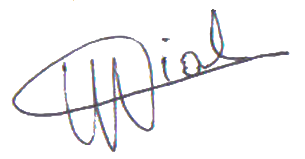
\includegraphics[width=3cm]{sig.png}
% 

\end{document}
